\newcommand{\FigSensMuMomentum}{
\begin{figure}[bt]
\centering 
\fbox{
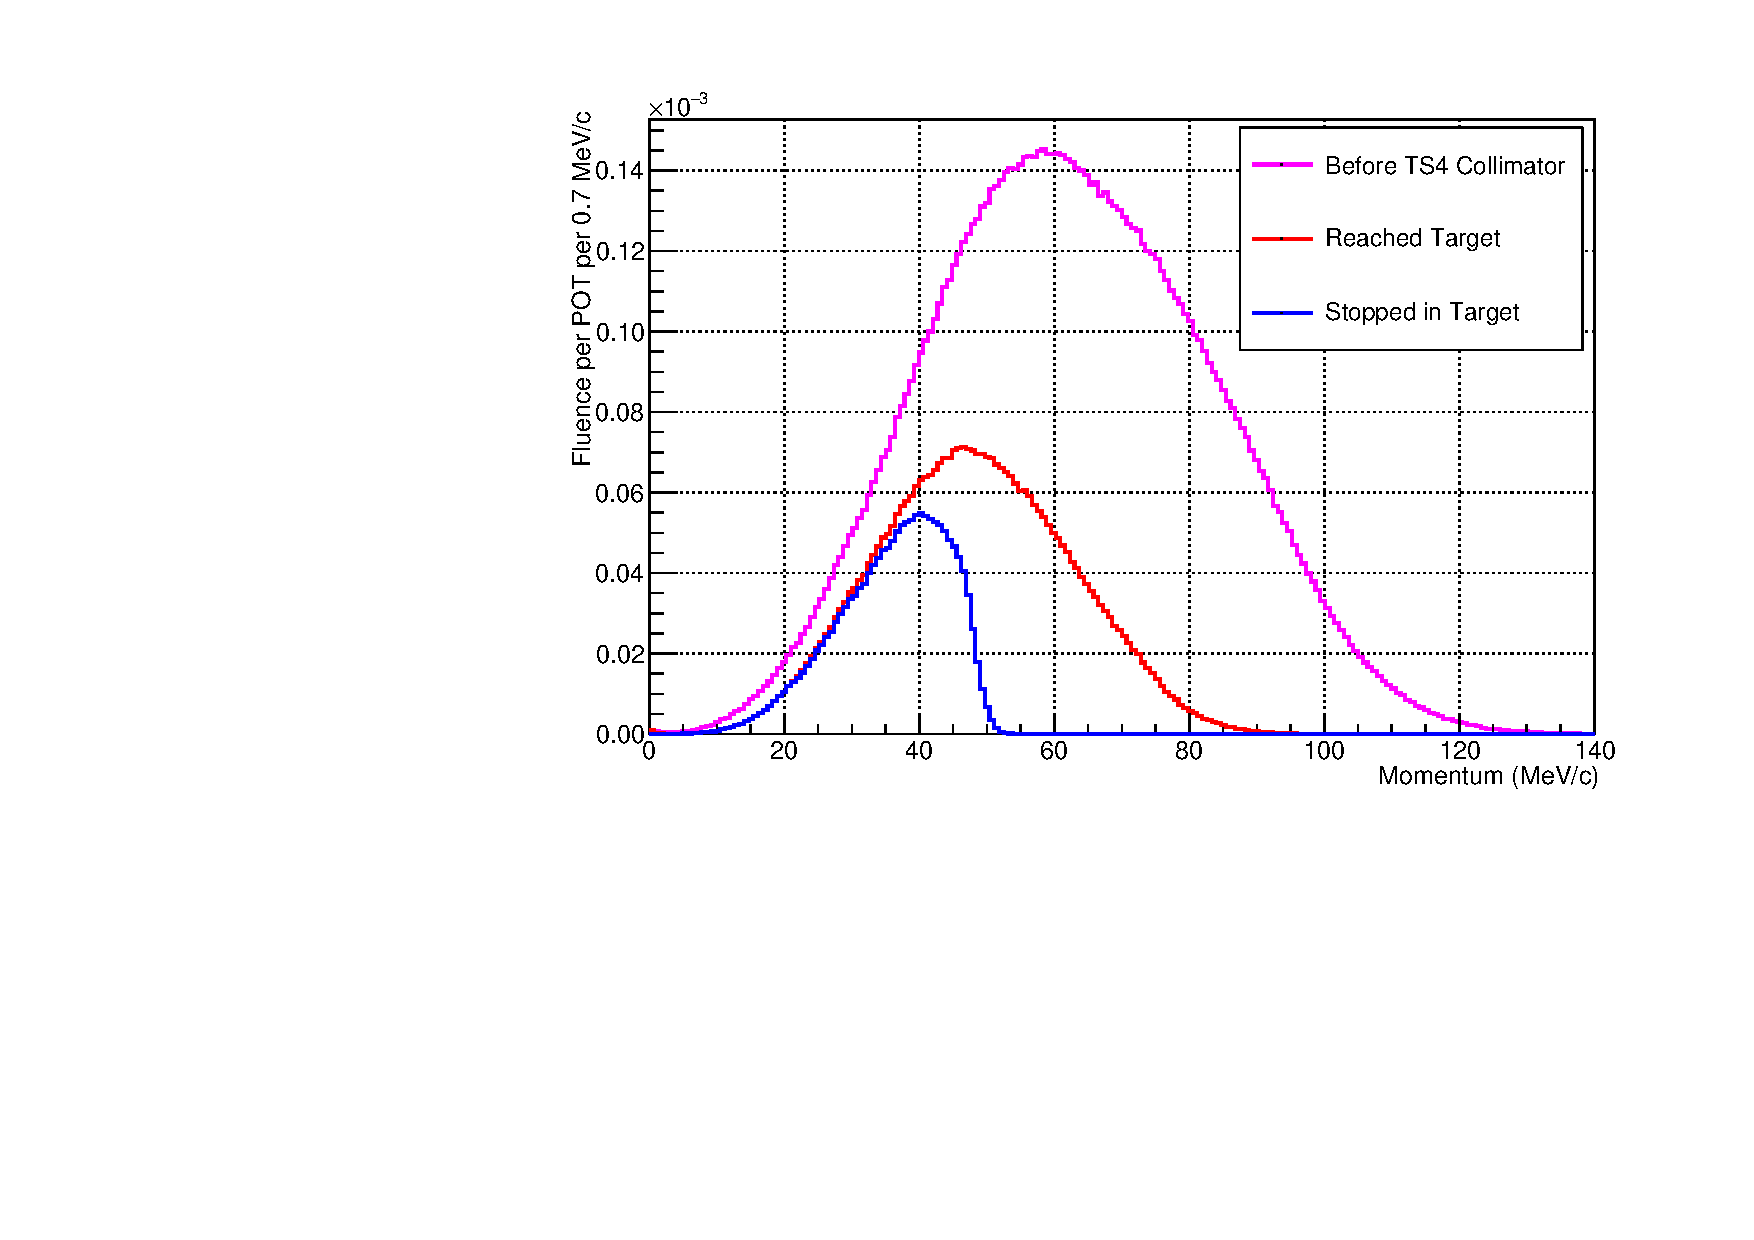
\includegraphics[width=0.8\textwidth,trim=0.5cm 0.1cm 1.5cm 0.8cm,clip]{figs/sensitivity/Muon_momentum.pdf}
}
\caption{\figlabel{sense:muMomenta}
The Momentum and rates of muons reaching the final beam collimator, the stopping target, and actually stopping in the target.
It can be seen how the present target geometry is unable to stop muons of greater than around 50~MeV/c.
}
\end{figure}
}

\newcommand{\FigSensMuStopsTwoD}{
\begin{figure}[tb]
\centering 
\subfloat[\figlabel{sense:stops2D:ZY}Z-Y plane]{
	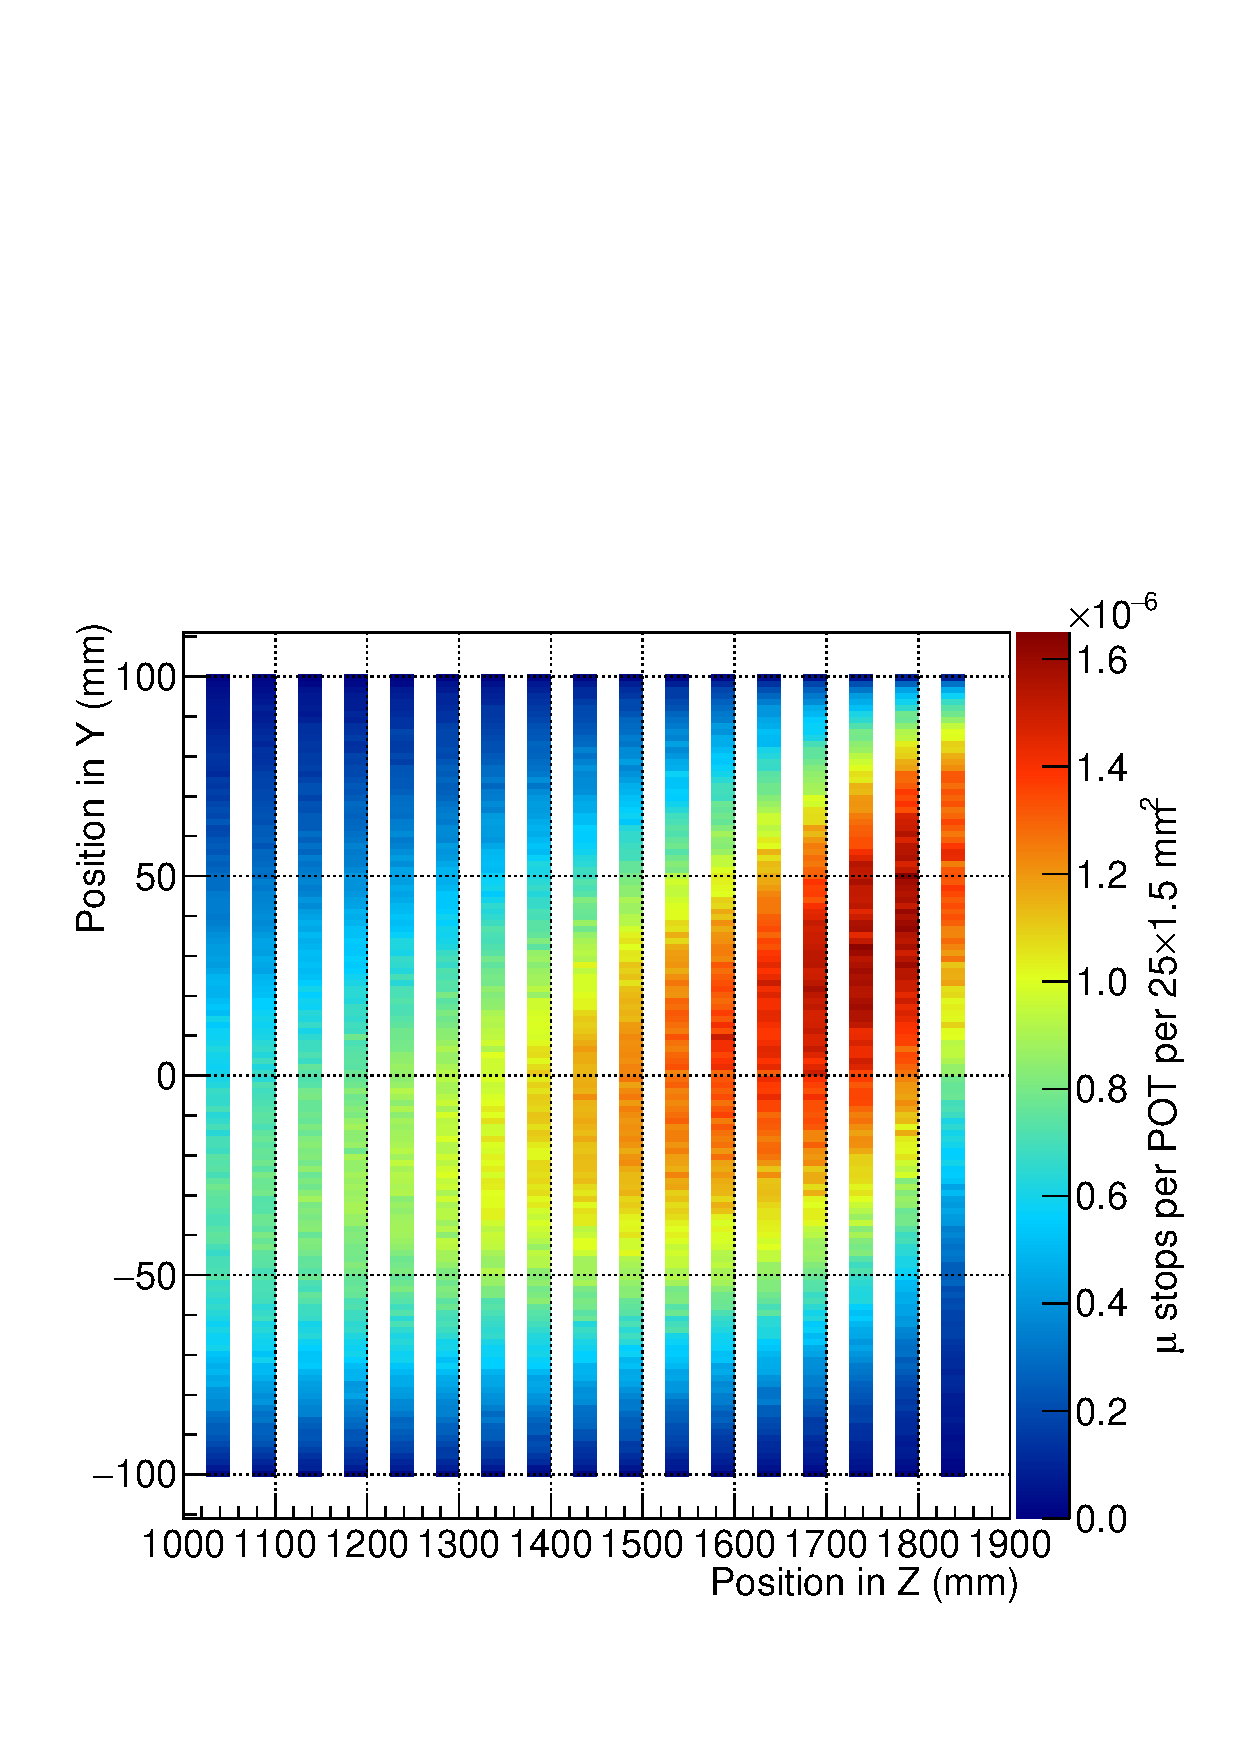
\includegraphics[width=0.33\textwidth,trim=0.3cm 1.5cm 0.7cm 1.2cm,clip]{figs/sensitivity/MuStops_2D_ZY.pdf}}
\subfloat[\figlabel{sense:stops2D:XY}X-Y plane]{
	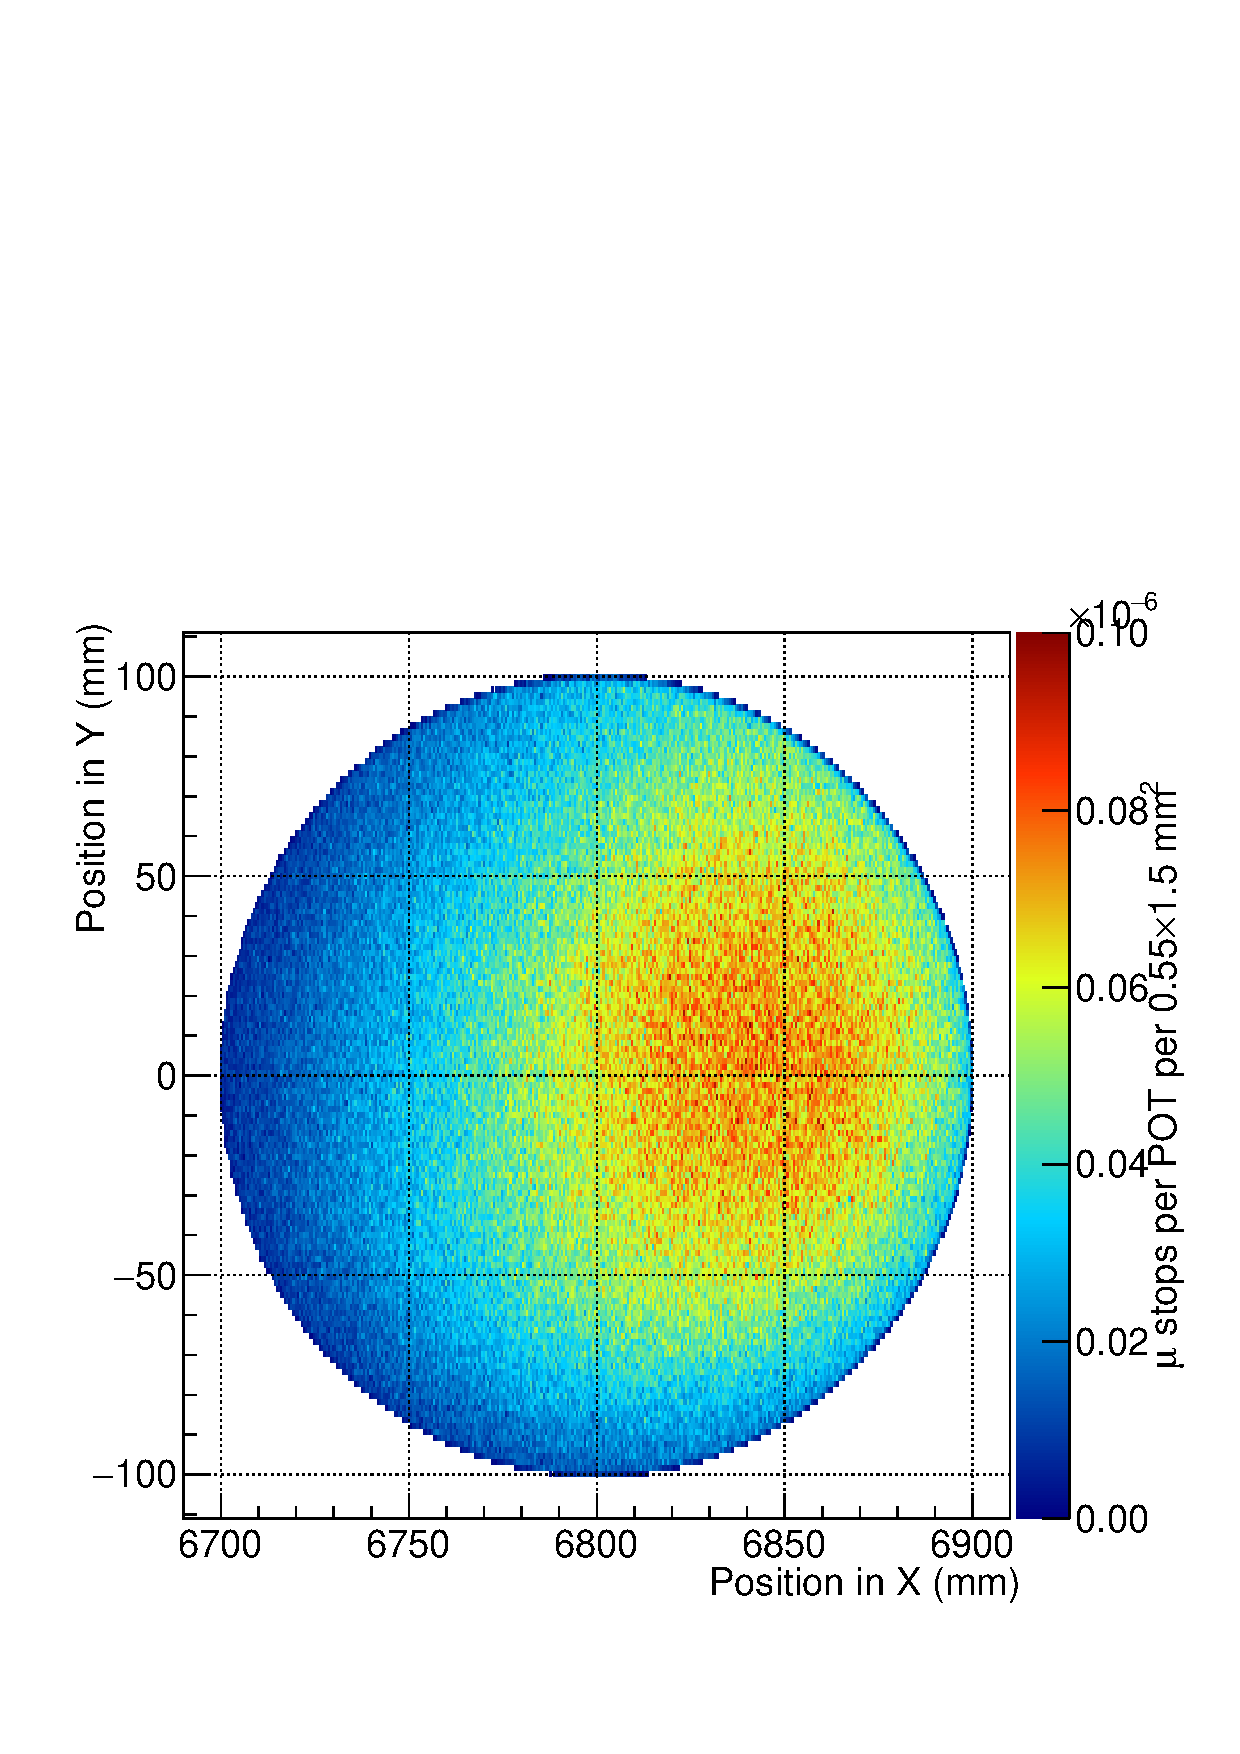
\includegraphics[width=0.33\textwidth,trim=0.3cm 1.5cm 0.7cm 1.2cm,clip]{figs/sensitivity/MuStops_2D_XY.pdf}}
\subfloat[\figlabel{sense:stops2D:XZ}X-Z plane]{
        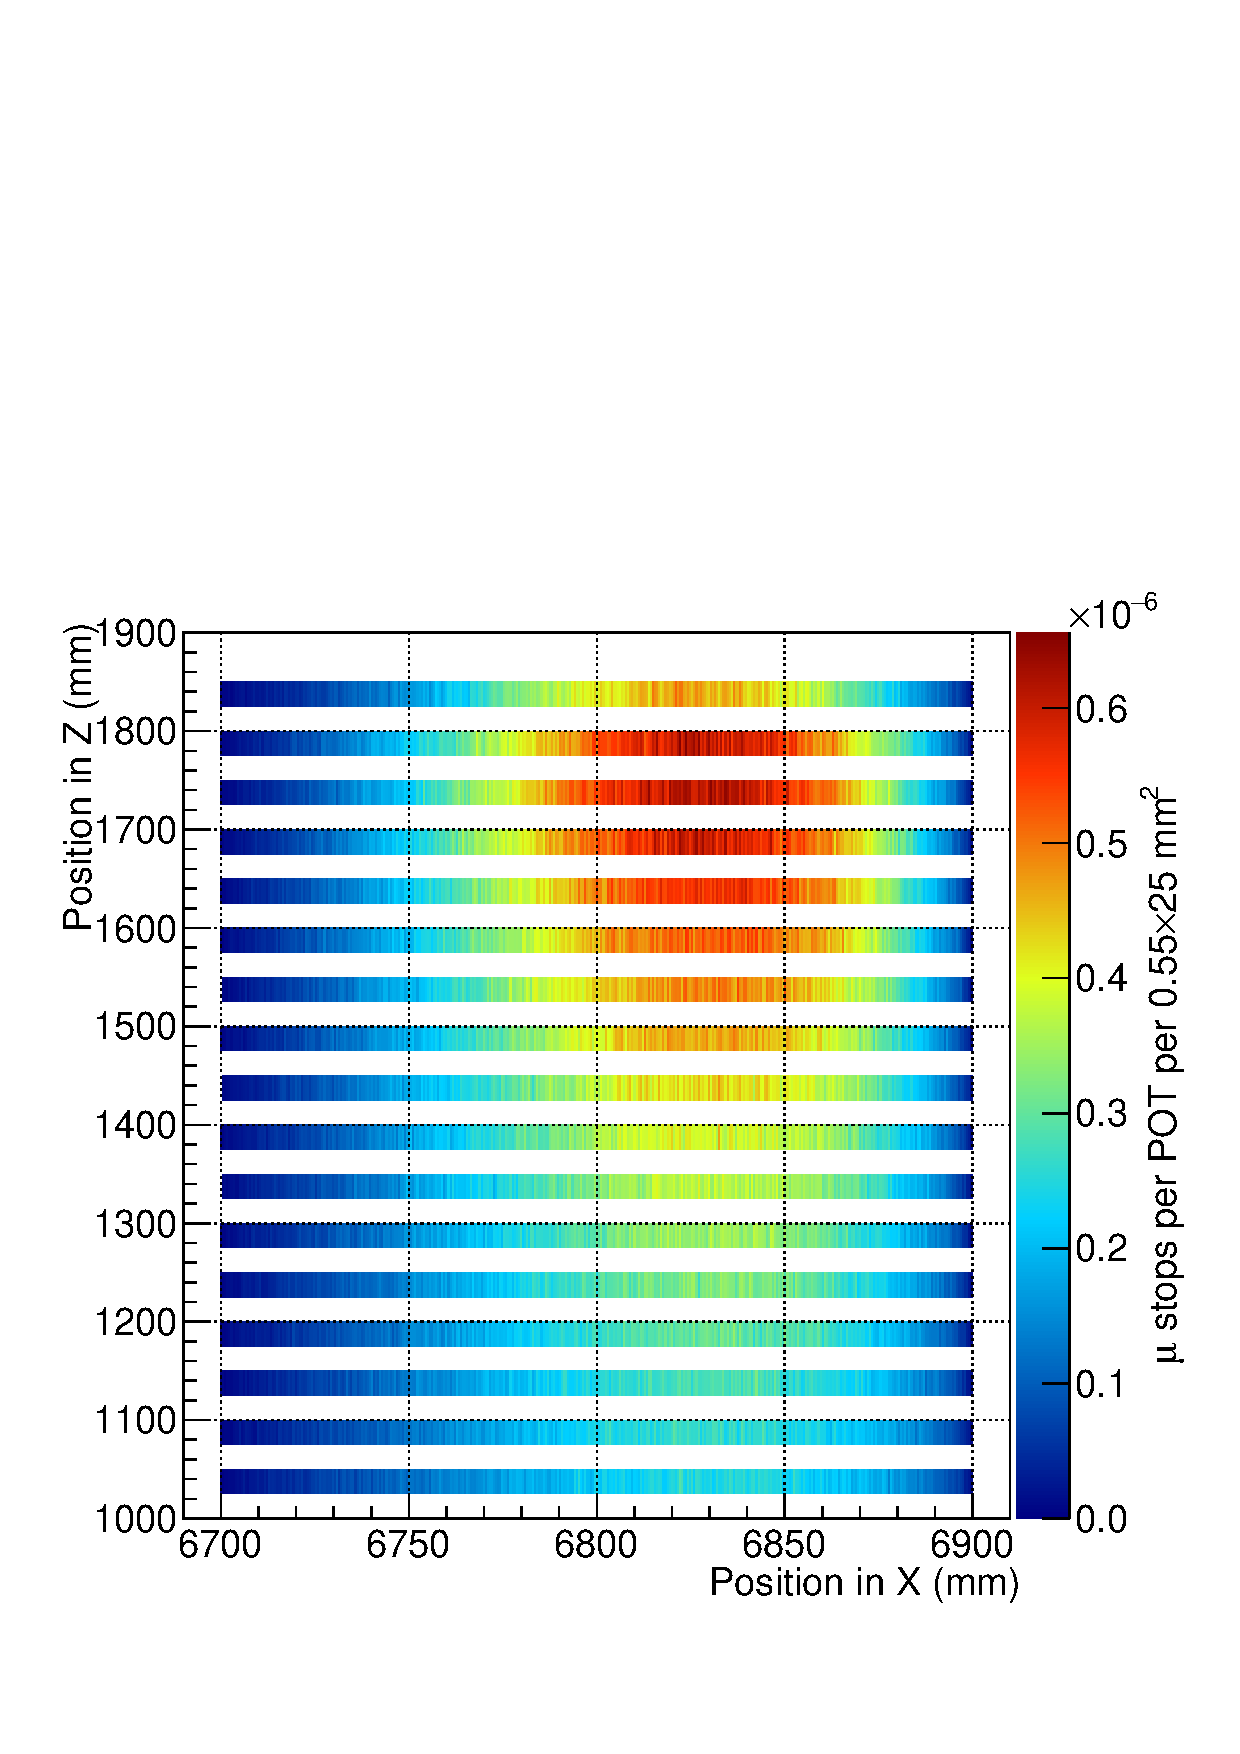
\includegraphics[width=0.33\textwidth,trim=0.3cm 1.5cm 0.7cm 1.2cm,clip]{figs/sensitivity/MuStops_2D_XZ.pdf}}
\caption{\figlabel{sense:stops2D}
Projections of the final position of stopped muons in the stopping target.
	Axes are from the SimG4 global coordinate system, so that $+X$ points away from the production target, $+Y$ is vertically upwards, and $+Z$ is the direction of the muon beam at the production target.
	The muon beam in these plots is therefore travelling in the negative-$Z$ direction since it has travlled 180\degree around the bent solenoid.
}
\end{figure}
}

\newcommand{\FigSensGeomAccept}{
\begin{figure}[tb]
\centering 
\subfloat[\figlabel{sense:accept:height}Path of Signal Electrons in the Beamline Projection]{
	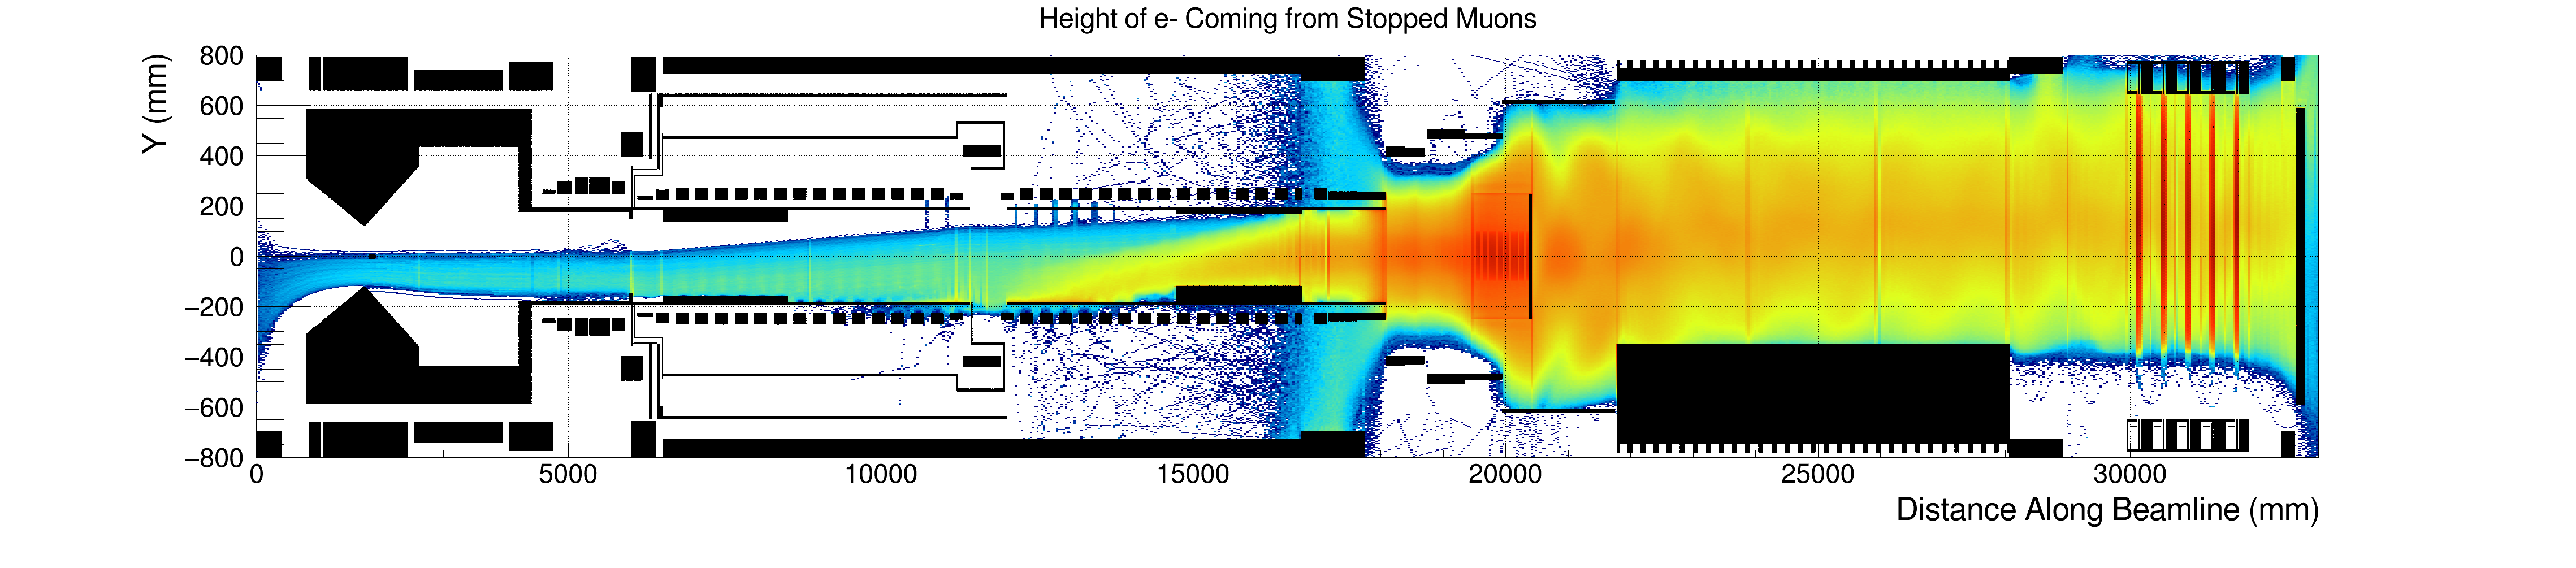
\includegraphics[width=0.99\textwidth,trim=8.3cm 1.5cm 13.2cm 2.2cm,clip]{figs/sensitivity/Tidied_SignalHeight2DVsBeamline.png}}\\
\subfloat[\figlabel{sense:accept:flux}Survival Probability for Signal Electrons]{
        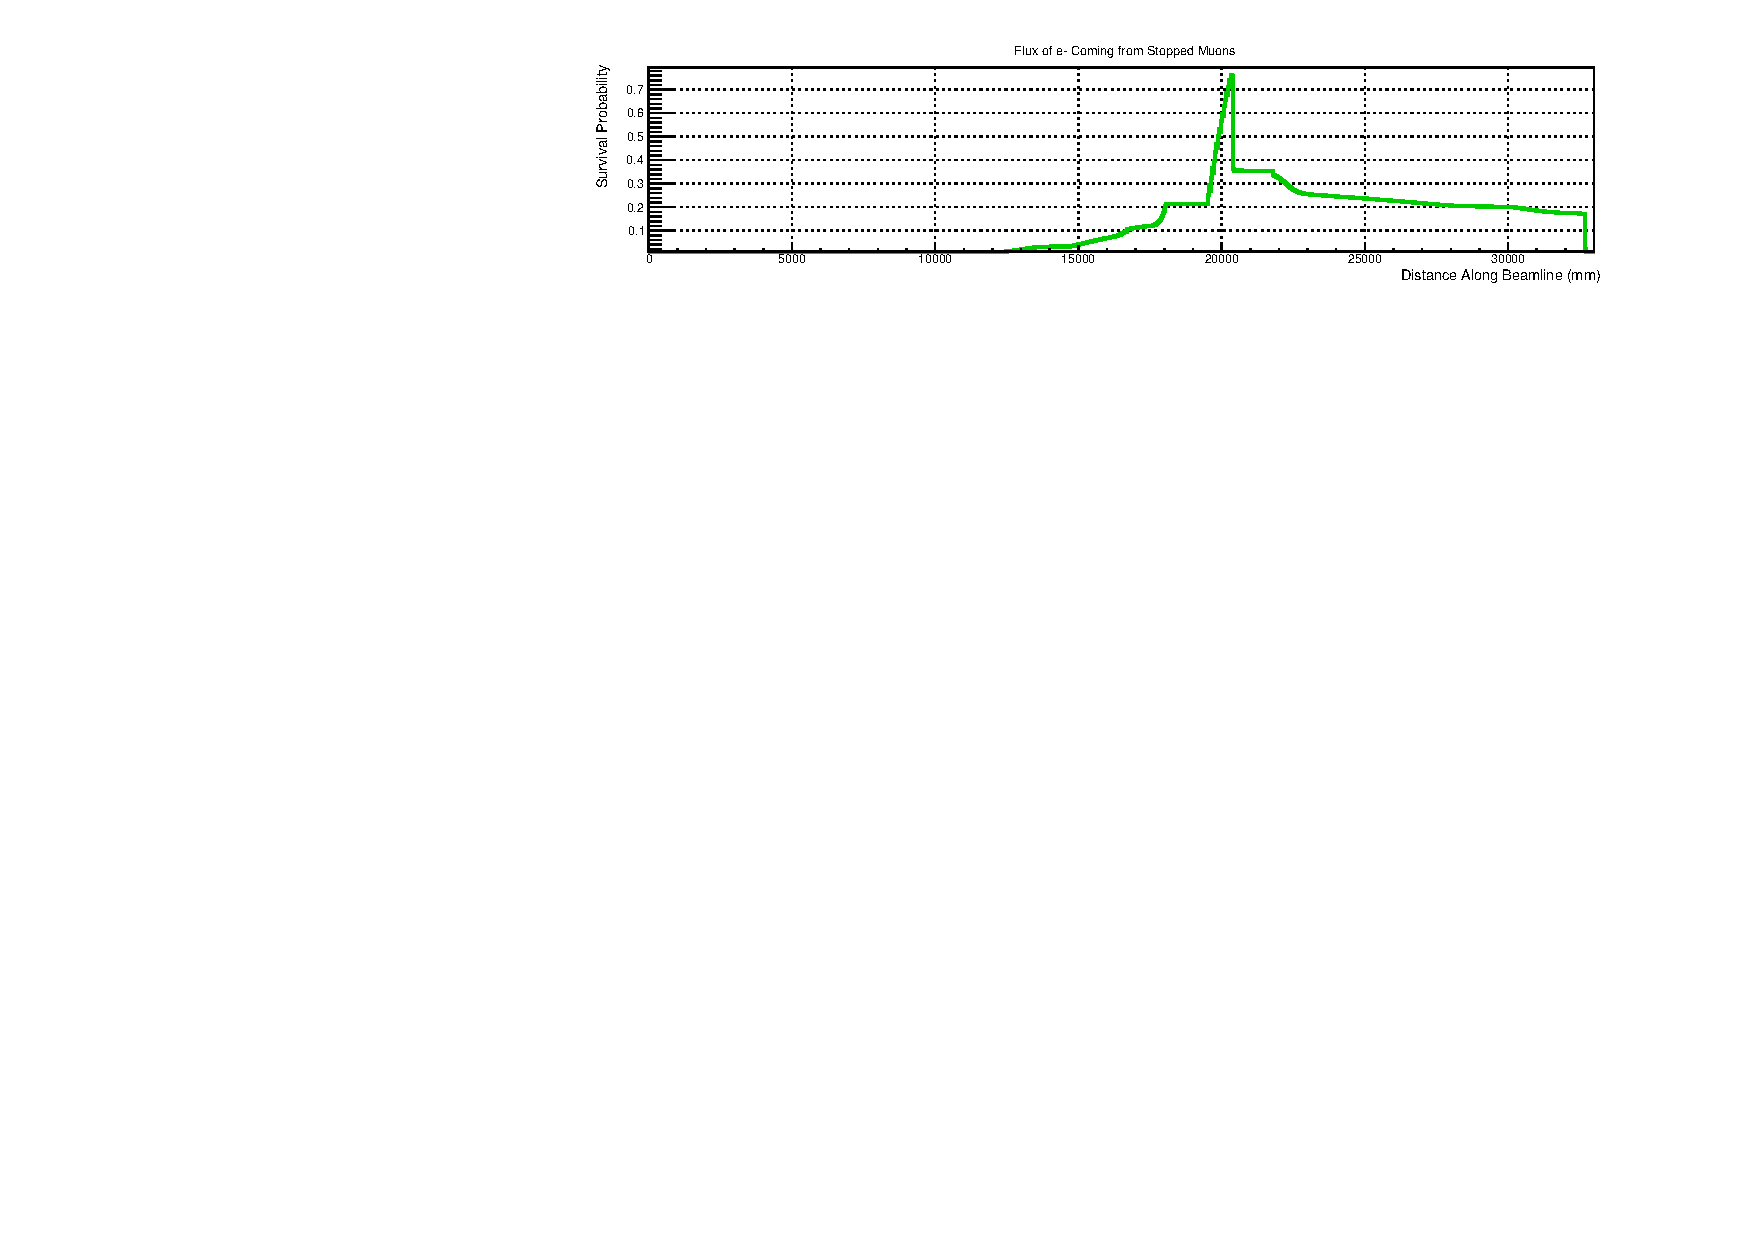
\includegraphics[width=0.99\textwidth,trim=1.0cm 0.2cm 1.7cm 0.4cm,clip]{figs/sensitivity/Tidied_SignalSurivivalVsBeamline.pdf}}
\caption{\figlabel{sense:accept}
Geometric acceptance of signal events.
\protect\subref{fig:sense:accept:height} Projection of the trajectories of signal electrons to the beamline axis-vertical surface.
\protect\subref{fig:sense:accept:flux} Survival probability of signal electrons as a function of the distance along the beamline axis.
From these plots it is clear how the acceptance is diminished by the DIO blocker in the spectrometer, although after the initial few hundred millimetres of blocker the rate of signal loss reduces.
}
\end{figure}
}

\newcommand{\FigSensMomTransfer}{
\begin{figure}[tb]
\centering 
%\fbox{
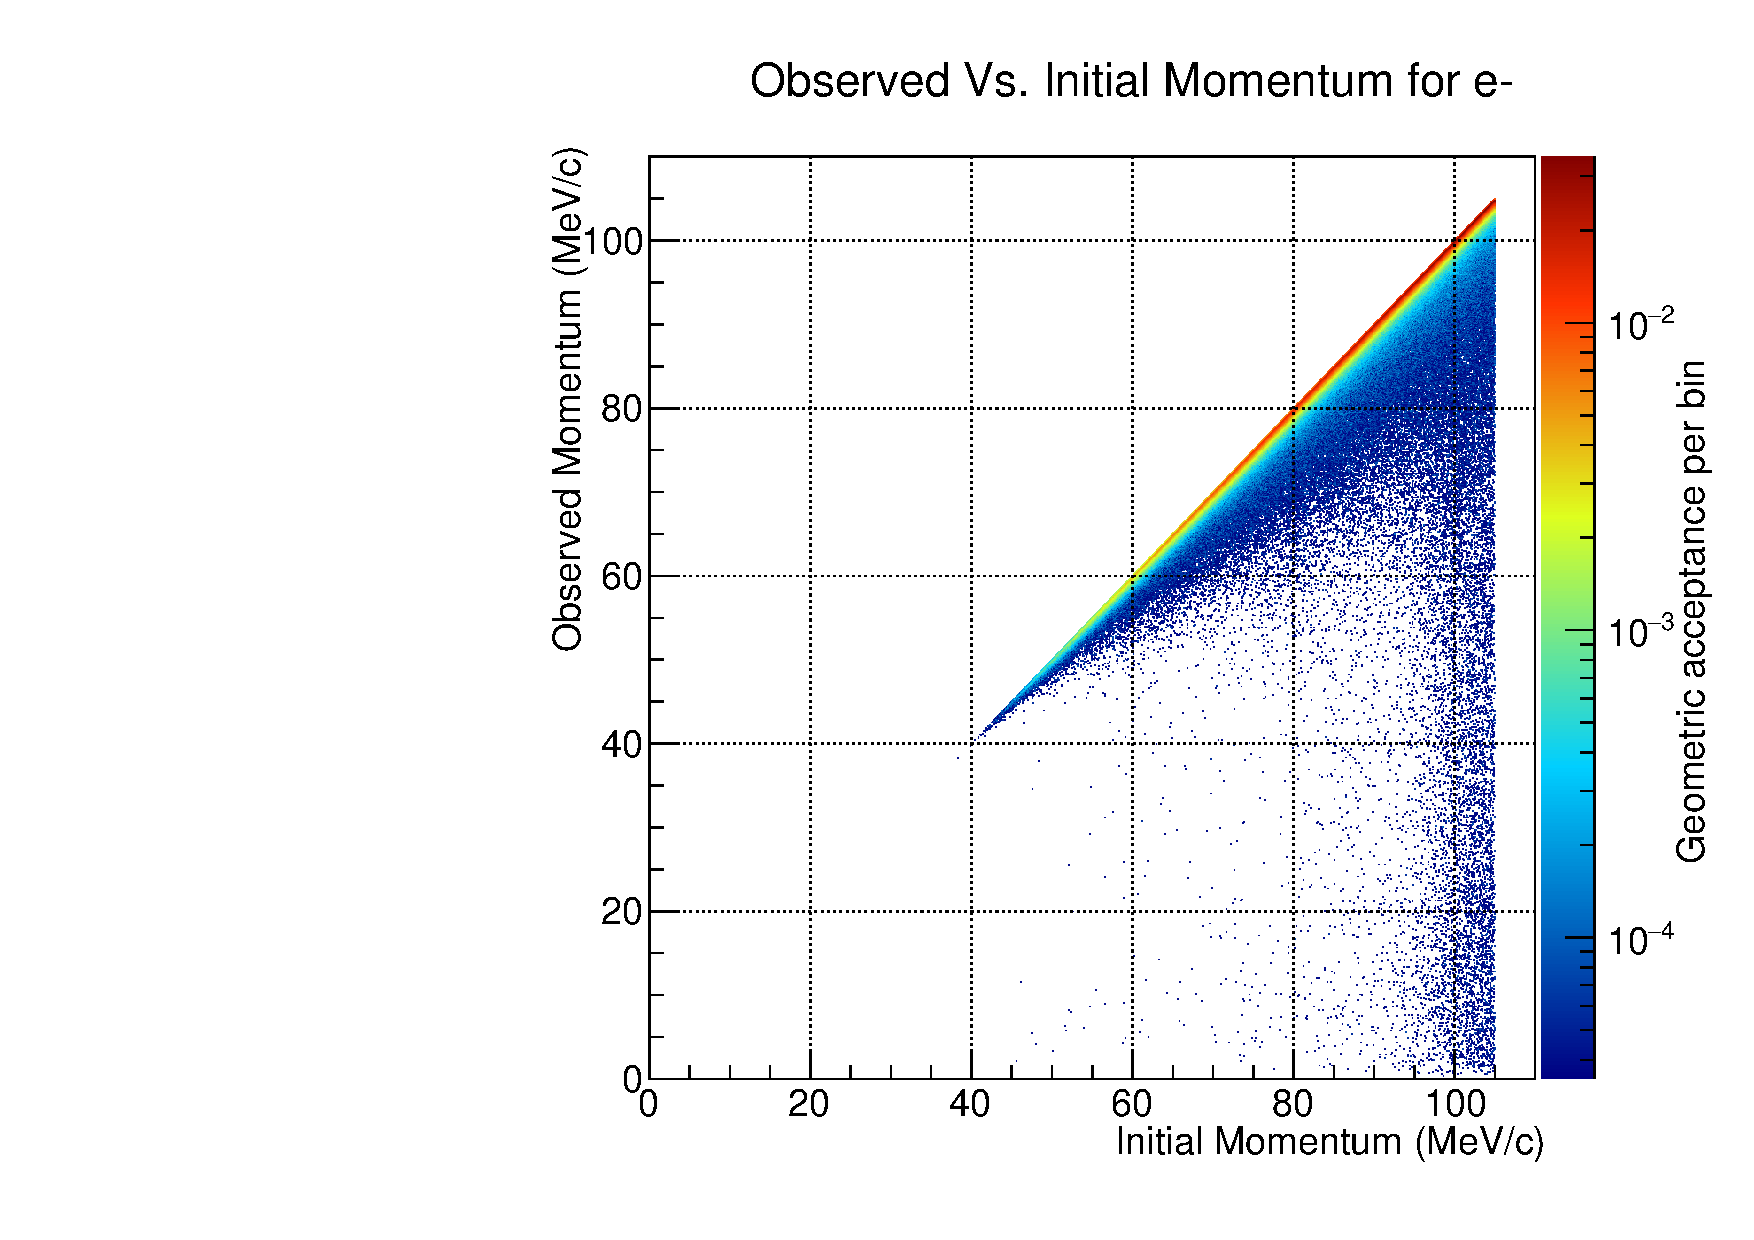
\includegraphics[width=0.5\textwidth,trim=0.0cm 0.0cm 0.0cm 1.6cm,clip]{figs/sensitivity/MomentumTransfer.pdf}
%}
\caption{\figlabel{sense:momTransfer}
The transfer matrix for electrons originating at the target, including the geometric acceptance and energy loss.
}
\end{figure}
}

\newcommand{\FigSensMomSpectra}{
\begin{figure}[tb]
\centering 
%\fbox{
\subfloat[\figlabel{sense:spectra:ELoss}Incl.~energy loss]             {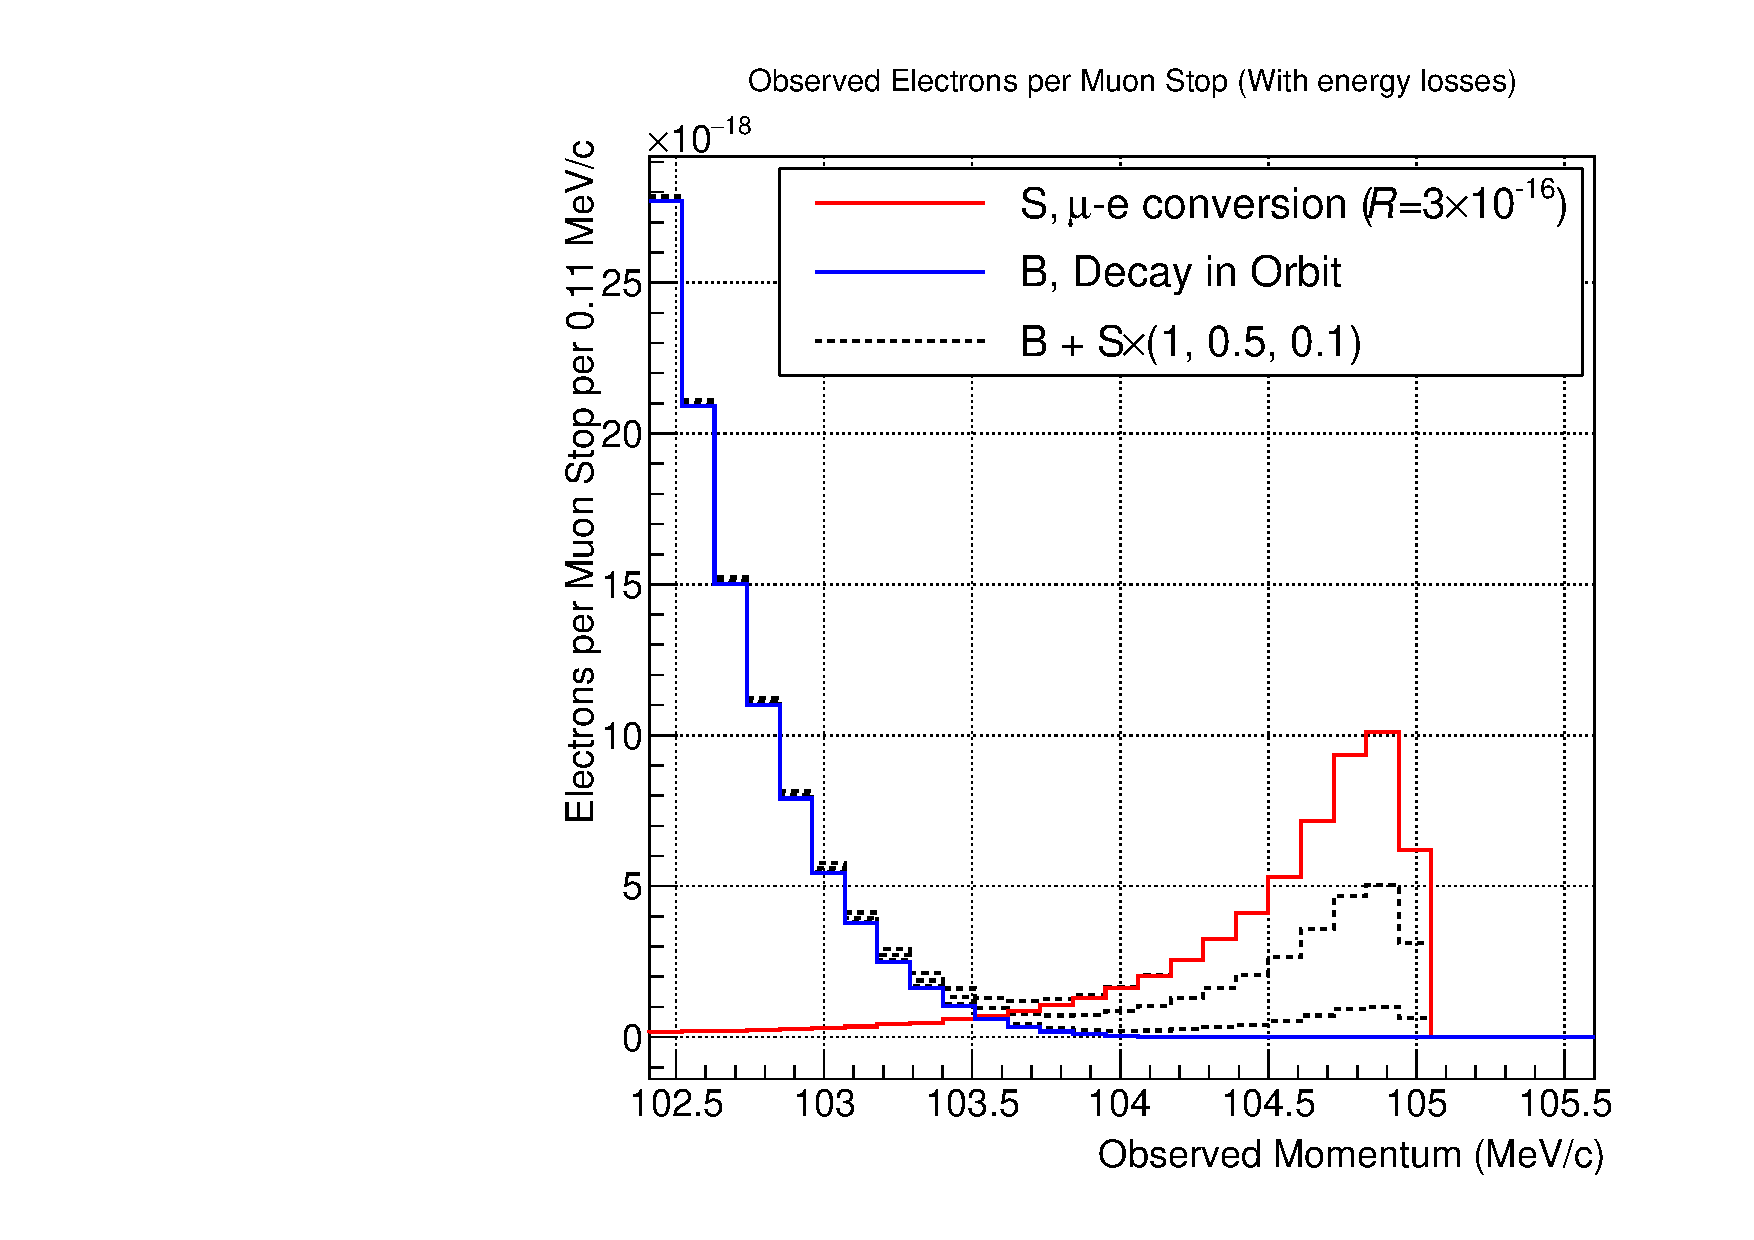
\includegraphics[width=0.48\textwidth,trim=0.0cm 0.0cm 1.0cm 1.0cm,clip]{figs/sensitivity/ConversionVsDio_Spectra.pdf}}
\subfloat[\figlabel{sense:spectra:resolution}Energy loss \& resolution]{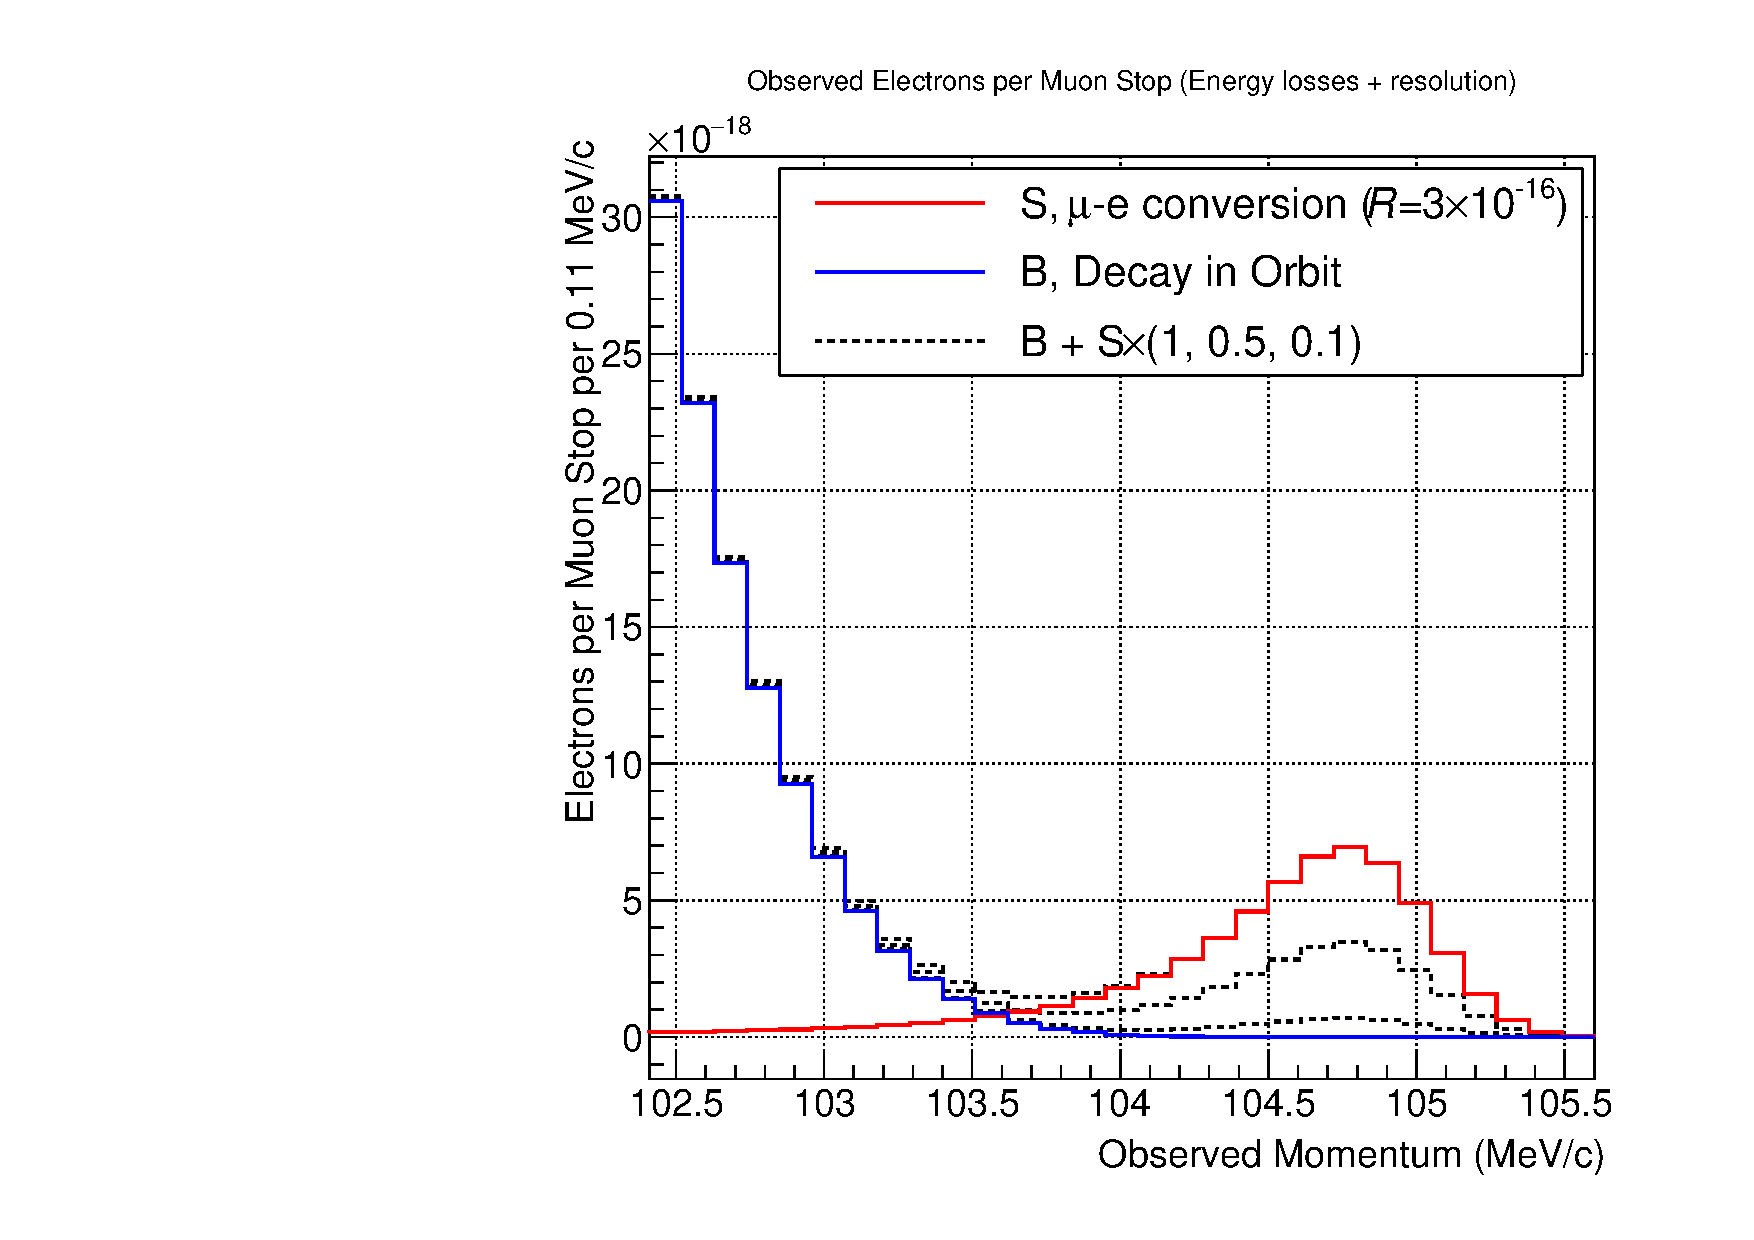
\includegraphics[width=0.48\textwidth,trim=0.0cm 0.0cm 1.0cm 1.0cm,clip]{figs/sensitivity/ConversionVsDio_Spectra-wResolution.pdf}}
\caption{\figlabel{sense:spectra}
The spectrum of electrons coming from \ac{DIO} and \mueconv assuming a conversion rate of $\mathcal{R}=\sci{3}{-16}$.
\protect\subref{fig:sense:spectra:ELoss} Includes energy losses in the target, beamline, and detector;
\protect\subref{fig:sense:spectra:resolution} also includes resolution effects (assumed the resolution function is perfect gaussian with a width of $\sigma=200$~keV/c).
}
\end{figure}
}

\newcommand{\FigSensMomIntegral}{
\begin{figure}[tb]
\centering 
%\fbox{
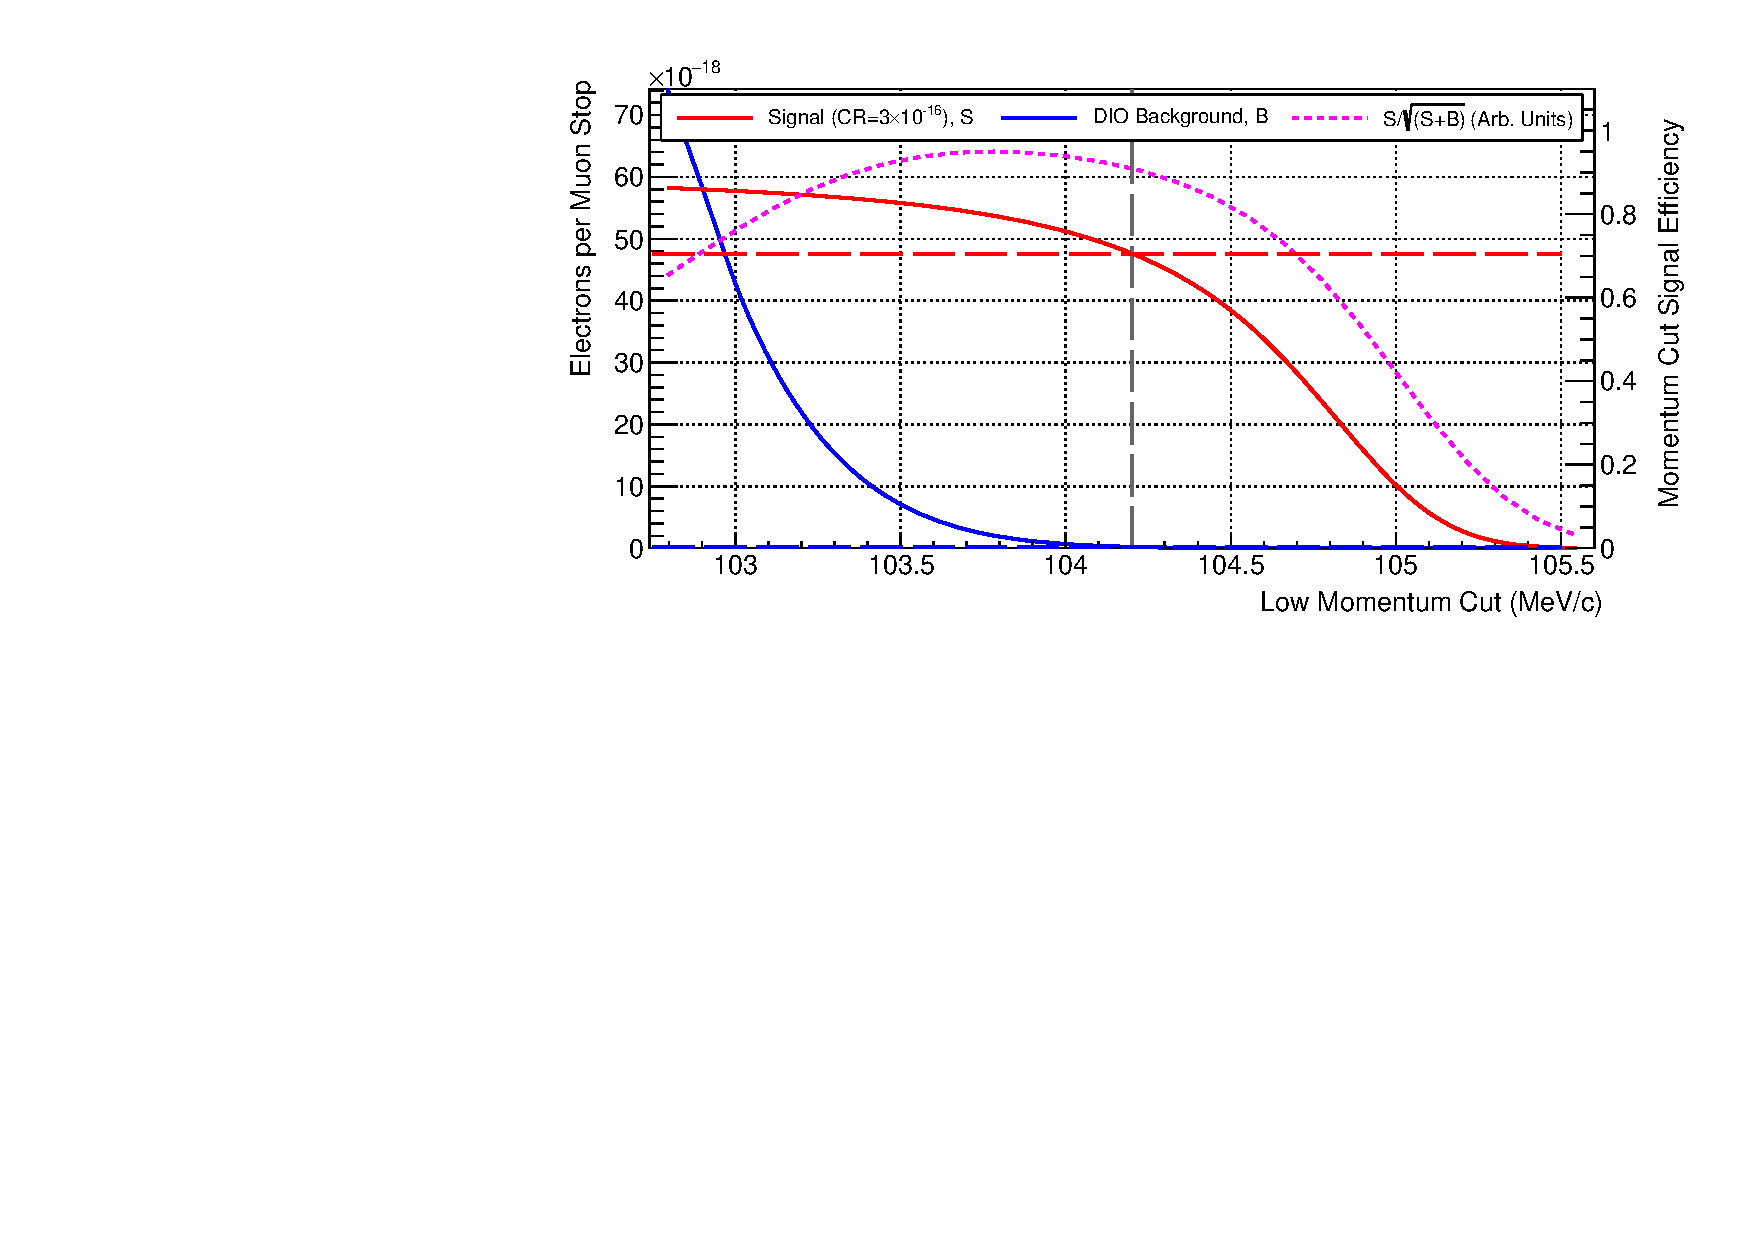
\includegraphics[width=0.99\textwidth,trim=1.0cm 0.0cm 1.0cm 0.6cm,clip]{figs/sensitivity/ConversionVsDio_Integrated.pdf}
%}
\caption{\figlabel{sense:integral}
Relative signal versus \ac{DIO} background as a function of the low momentum cut value assuming a conversion rate of $\mathcal{R}=\sci{3}{-16}$.
The magenta line is the signal over square root of signal plus background for this conversion rate shown as an indicator of the optimum cut value.
}
\end{figure}
}

\newcommand{\FigSensTiming}{
\begin{figure}[b]
\centering 
%\fbox{
\subfloat[\figlabel{sense:timing:signal}Signal Arrival Time]      {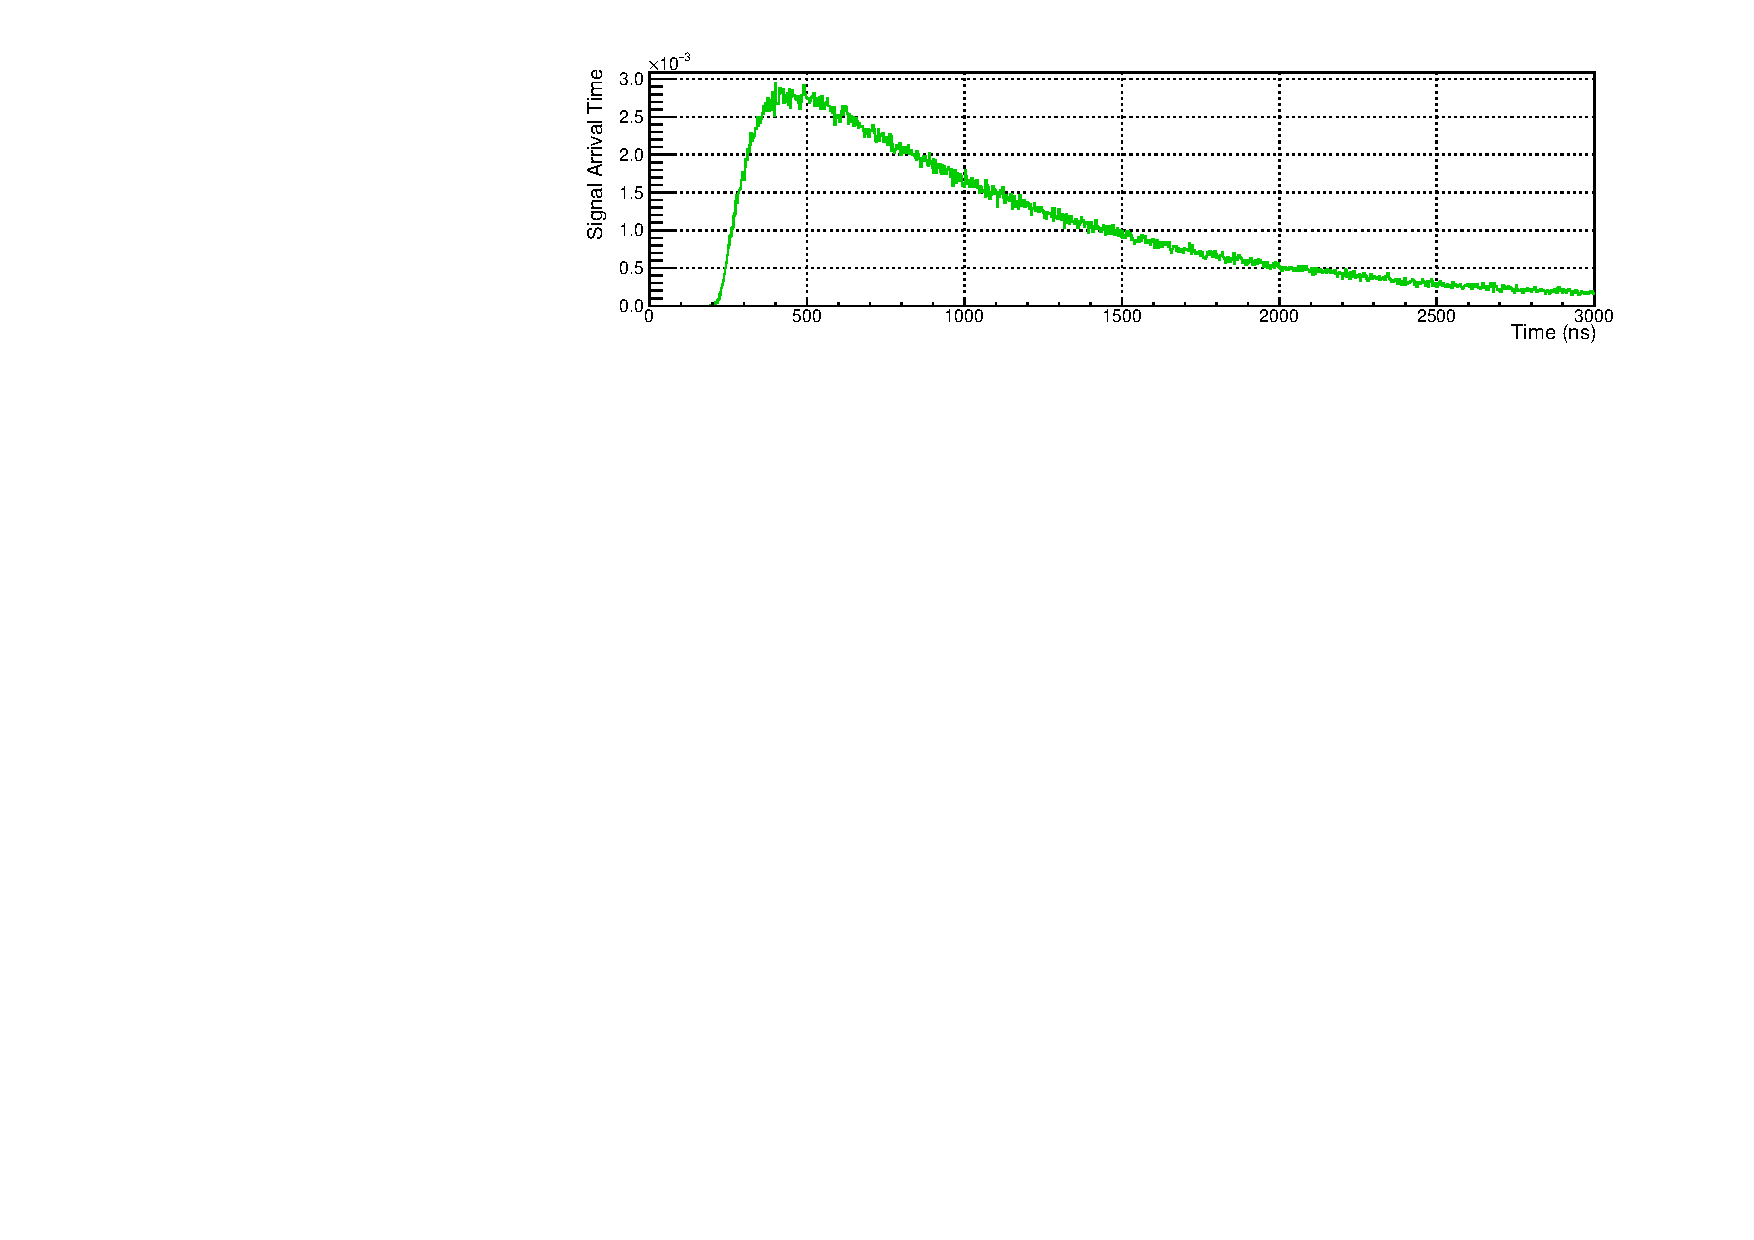
\includegraphics[width=0.9\textwidth,trim=0.9cm 0.1cm 1.5cm 0.20cm,clip]{figs/sensitivity/160823_MuonLifetime.pdf}}\\
\subfloat[\figlabel{sense:timing:efficiency}Timing Cut Efficiency]{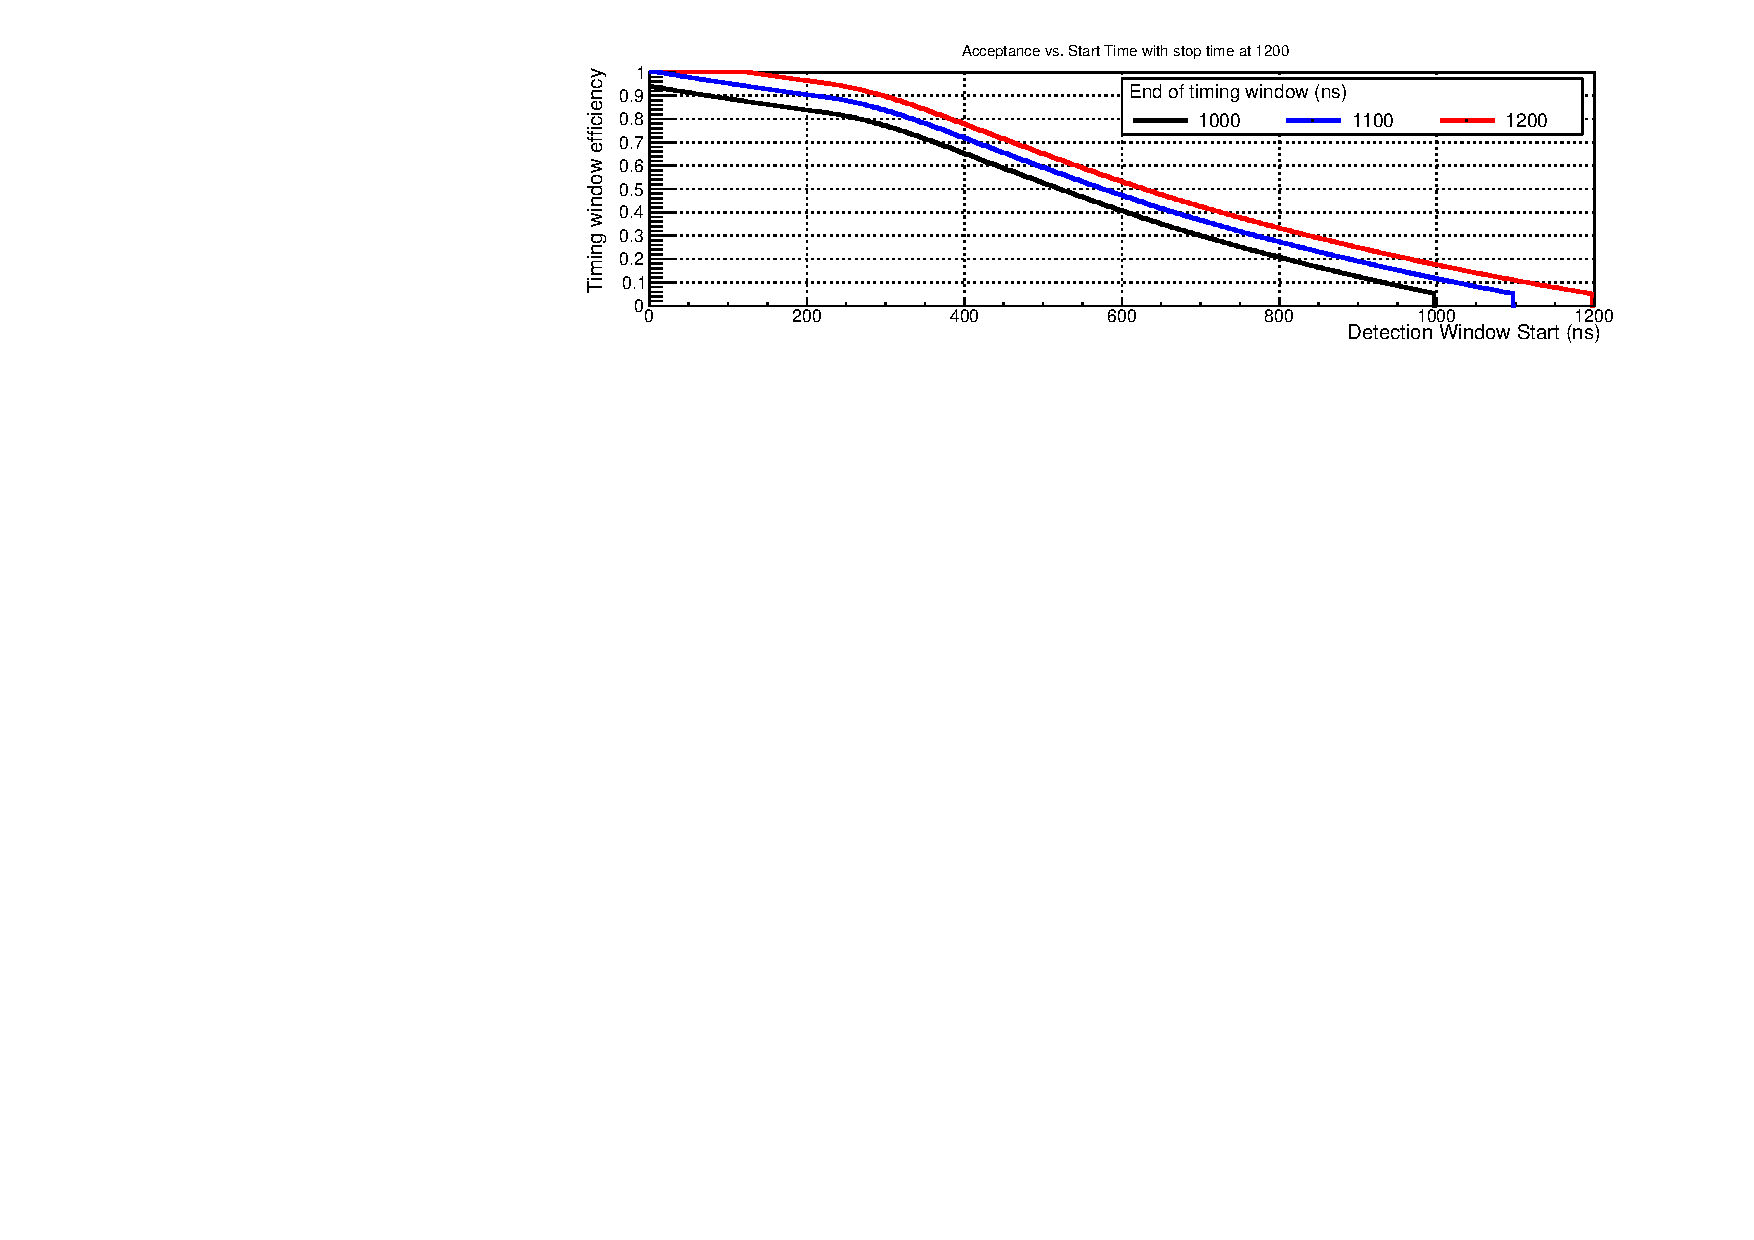
\includegraphics[width=0.9\textwidth,trim=0.9cm 0.1cm 1.5cm 0.4cm,clip]{figs/sensitivity/160823_TimingCutEfficiency.pdf}}
\caption{\figlabel{sense:timing}
Timing of signal electrons.
\protect\subref{fig:sense:timing:signal} The arrival time of signal electrons at the detector, including the effect of the proton pulse width, particle transportation, and the muon lifetime.
\protect\subref{fig:sense:timing:efficiency} the efficiency of the timing window as a function of the switch-on time.  Assumes a pulse separation of 1.17~$\mu$s.
}
\end{figure}
}

